\documentclass[a4paper,12pt]{article}

\usepackage{amsmath,amssymb,multicol,tikz,enumitem}
\usepackage[margin=2cm]{geometry}
\usetikzlibrary{calc,shapes}

\pagestyle{empty}

\newcommand\N{\mathbf{N}}
\newcommand\Q{\mathbf{Q}}
\newcommand\R{\mathbf{R}}
\newcommand\Z{\mathbf{Z}}

\usepackage{array}
\newcolumntype{P}[1]{>{\centering\arraybackslash}p{#1}}
\newcommand\indd{${}$\hspace{20pt}}

\begin{document}

\begin{center}
\parbox{3.5cm}{\textbf{Data Structures}} \hfill {\bf\Huge Worksheet 7} \hfill \parbox{3.5cm}{\flushright\textbf{BITL2}} \\[5pt]
\rm\small 11 November 2021
\end{center}

\hrule\vspace{2pt}\hrule

\vspace{10pt}
\noindent
Recall several properties of graphs and the algorithms that compute them:
\begin{itemize}
\item \textbf{maxmimum flow:} The largest value to place on each edge, subject to edge and vertex conditions, to maximize flow from the source to the sink
\begin{itemize}
\item the \textit{Ford--Fullkerson algorithm} increases flow capacity along paths step by step until the maximum flow is reached on that path
\end{itemize}

\item \textbf{shortest path:} The path with the least weight between nodes
\begin{itemize}
\item \textit{Dijkstra's algorithm} does a breadth-first greedy search from a root node
\item the \textit{Bellman--Ford algorithm} recalculates distance to every edge at each step
\end{itemize}
\item \textbf{minimum spanning tree:} The smallest weight subtree that that spans the graph
\begin{itemize}
\item \textit{Kruskal's algorithm} builds clusters by adding minimal weight edges
\item \textit{Prim's algorithm} starts at a root node and adds minimal weight edges
\end{itemize}
\end{itemize}
\hrule

\begin{enumerate}

\item \textbf{Warm up:} Answer the following questions.
\begin{enumerate}
\item What does a connected graph for which BFS and DFS reaches a given node node in the same number of steps look like?
\item Is it possible to have a connected graph with two spanning trees that do not share any edges?
\item What condition on a binary tree will guarantee that it does not have a perfect matching?
\end{enumerate}

\item For the graph $G$ below, and the root node $0$, add weights to the edges so that the minimal spanning trees built by Kruskal's and Prim's algorithm share the least number of edges possible. The order of the vertices indicates the order in which they are considered for each algorithm.
\[
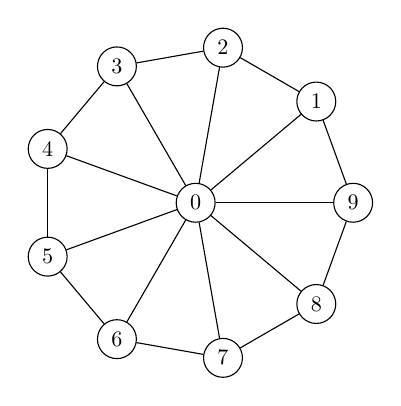
\begin{tikzpicture}
\node[circle,draw,scale=.8] (v) at (0,0) {$0$};
\foreach \r in {1,...,9}{
  \node[circle,draw,scale=.8] (\r) at ($(0,0)+(360/9*\r:2)$) (\r) {$\r$};
  \draw (v)--(\r);
}
\foreach \x\y in {1/2, 2/3, 3/4, 4/5, 5/6, 6/7, 7/8, 8/9, 9/1}{
  \draw(\x)--(\y);
}
\end{tikzpicture}
\]

\item Let $G=(V,E)$ be a graph with two different weight functions 
\[
w\colon E\to \Z,
\hspace{1cm}
w'\colon E\to \N\cup \{0\},
\]
with $w'(e) = w(e)-\min_{\varepsilon \in E}\{w(\varepsilon)\}$. Suppose that Bellman--Ford is run on $G$ with weights $w$, and Dijkstra is run on $G$ with weights $w'$. What is the relationship between the two resulting subgraphs?
\end{enumerate}

\end{document}